\chapter{Double Integrals Over Non-Rectangular Regions}


Now that we've seen how to evaluate double integrals over rectangular regions, 
let's consider non-rectangular regions. Suppose we are interested in the 
integral of a function, $f(x,y)$, over a region, \textit{D}, which exists such that 
it can be bounded by inside a rectangular region, \textit{R} (see figure 
\ref{fig:enclose}). We can then define a new function:
$$F(x, y) = 
\begin{cases}
	f(x, y) & \text{if } (x, y) \text{ is in \textit{D}}\\
	0 & \text{if } (x, y) \text{ is in \textit{R} but not in \textit{D}}
\end{cases}$$

\begin{figure}[htbp]
    \centering
    \begin{minipage}{0.45\textwidth}
        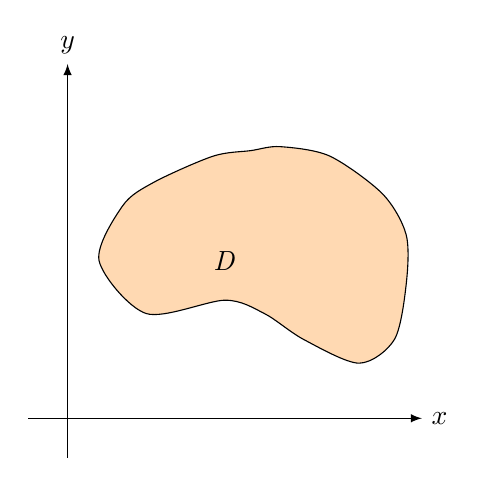
\begin{tikzpicture}
            \draw[-latex] (-0.5, 0) -- (4.5, 0) node[right] {$x$};
            \draw[-latex] (0, -0.5) -- (0, 4.5) node[above] {$y$};
            \draw[fill = orange!30] plot [smooth cycle] 
        coordinates {(0.4, 2) (0.7, 2.7) (1.1, 3) (1.85, 3.33) (2.33, 3.4) 
        (2.7, 3.45) (3.33, 3.33) (4, 2.85) (4.3, 2.33) (4.3, 1.7) (4.15, 1) 
        (3.7, 0.7) (3, 1) (2.5, 1.33) (2, 1.5) (1, 1.33)};
        \node[] at (2, 2) {\textit{D}};
        \end{tikzpicture}
    \end{minipage}
    \begin{minipage}{0.45\textwidth}
        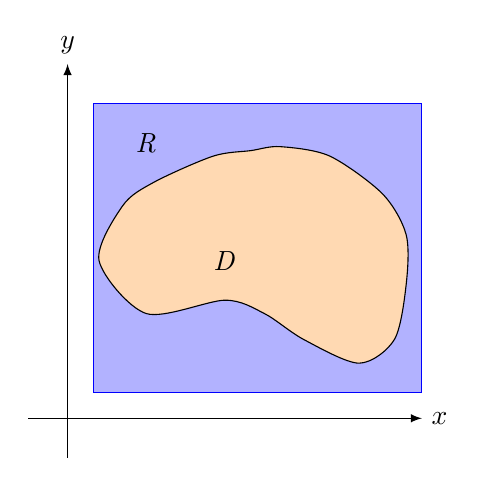
\begin{tikzpicture}
            \draw[-latex] (-0.5, 0) -- (4.5, 0) node[right] {$x$};
            \draw[-latex] (0, -0.5) -- (0, 4.5) node[above] {$y$};
            \draw[blue, fill = blue!30] (0.33, 0.33) rectangle (4.5, 4);
            \draw[fill = orange!30] plot [smooth cycle] 
        coordinates {(0.4, 2) (0.7, 2.7) (1.1, 3) (1.85, 3.33) (2.33, 3.4) 
        (2.7, 3.45) (3.33, 3.33) (4, 2.85) (4.3, 2.33) (4.3, 1.7) (4.15, 1) 
        (3.7, 0.7) (3, 1) (2.5, 1.33) (2, 1.5) (1, 1.33)};
        \node[] at (2, 2) {\textit{D}};
        \node[] at (1, 3.5) {\textit{R}};
        \end{tikzpicture}
    \end{minipage}
    \caption{We can find a rectangular region, \textit{R}, that completely 
    encloses \textit{D}}
    \label{fig:enclose}
\end{figure}

Then, we can see that:
$$\iint_{\textit{D}} f(x, y)\,dA = \iint_{\textit{R}} F(x, y)\,dA$$

This makes sense intuitively, since integrating over $F$ outside of \textit{D}
doesn't contribute anything to the integral, and the integral of $F$ inside 
\textit{D} is equal to the integral of $f$ inside \textit{D}. In general, there
are two types of regions for \textit{D}. A region is \textbf{type I} if it lies
between two continuous functions of $x$ and can be defined thusly:
$$\textit{D} = \{ (x, y) \text{ } | \text{ } a \leq x \leq b, g_1(x) \leq y 
\leq g_2(x) \}$$

\begin{figure}[htbp]
    \centering
    \begin{minipage}{0.5\textwidth}
        \begin{tikzpicture}
            \begin{axis}[ymin = -0.3, ymax = 4, xmin = -0.3, xmax = 3, 
            axis lines = center, ticks = none, xlabel = $x$, ylabel = $y$] 
                \addplot[name path = A, domain = 0.5:2.5, orange, thick] {
                (0.5*x - 0.75)^2 + 0.5};
                \addplot[name path = B, domain = 0.5:2.5, orange, thick] {
                (x-2)^3 + 2*(x-2)^2 + x -1 + 1.5};
                \addplot[fill = orange!30] fill between [of = A and B];
                \draw[orange, thick] (0.5, 0.75) -- (0.5, 2.12);
                \draw[orange, thick] (2.5, 0.75) -- (2.5, 3.65);
                \draw[dashed] (0.5, 0.75) -- (0.5, 0) node[below] {$a$};
                \draw[dashed] (2.5, 0.75) -- (2.5, 0) node[below] {$b$};
                \node[] at (1.5, 2.8) {$y = g_2 (x)$};
                \node[] at (1.75, 0.25) {$y = g_1 (x)$};
                \node[] at (1.5, 1.5) {\textit{D}};
            \end{axis}
        \end{tikzpicture}
    \end{minipage}
    
    \begin{minipage}{0.5\textwidth}
        \begin{tikzpicture}
            \begin{axis}[ymin = -0.3, ymax = 4, xmin = -0.3, xmax = 3, 
            axis lines = center, ticks = none, xlabel = $x$, ylabel = $y$] 
                \addplot[name path = A, domain = 0.5:2.5, orange, thick, 
                samples = 150] {1.75 + sqrt(x - 0.5)};
                \addplot[name path = B, domain = 0.5:2.5, orange, thick, 
                samples = 150] {1.75 - sqrt(x - 0.5)};
                \addplot[fill = orange!30] fill between [of = A and B];
                \draw[orange, thick] (2.5, 0.33) -- (2.5, 3.17);
                \draw[dashed] (0.5, 1.75) -- (0.5, 0) node[below] {$a$};
                \draw[dashed] (2.5, 0.33) -- (2.5, 0) node[below] {$b$};
                \node[] at (1.25, 3.1) {$y = g_2 (x)$};
                \node[] at (1.5, 0.25) {$y = g_1 (x)$};
                \node[] at (1.5, 1.5) {\textit{D}};
            \end{axis}
        \end{tikzpicture}
    \end{minipage}
    \caption{Two examples of type I domains}
    \label{fig:type1}
\end{figure}

Some type I regions are shown in figure \ref{fig:type1}. To evaluate $\iint_{
\textit{D}} f(x,y)\,dA$, we begin by choosing a rectangle $\textit{R} = \left[ 
a, b \right] \times \left[ c, d \right]$ such that \textit{D} is completely 
contained in \textit{R}. We again define $F(x, y)$ such that $F(x, y) = f(x,y)$
on \textit{D} and $F = 0$ outside of \textit{D}. Then, by Fubini's theorem:
$$\iint_{\textit{D}} f(x, y)\,dA = \iint_{\textit{R}} F(x, y)\,dA = \int_a^b 
\int_c^d F(x, y)\,dy\,dx$$

Since $F(x, y) = 0$ when $y \leq g_1(x)$ or $y \geq g_2(x)$, we know that:
$$\int_c^d F(x, y)\,dy = \int_{g_1(x)}^{g_2(x)} F(x, y)\,dy = \int_{g_1(x)}^{
g_2(x)} f(x, y)\,dy$$

Substituting this into the iterated integral above, we see that for a type I 
region $\textit{D} = \{ (x, y) \text{ } | \text{ } a \leq x \leq b, g_1(x) 
\leq y \leq g_2(x) \}$, 
$$\iint_{\textit{D}} f(x, y)\,dA = \int_a^b \int_{g_1(x)}^{g_2(x)} f(x, y)
\,dy\,dx$$

Another way to visualize the double integral over a type I region is shown in 
figure \ref{fig:direction_typeI}. For any value of $x \in \left[ a, b 
\right]$, we know that $g_1(x) \leq y \leq g_2(x)$. The inner integral 
represents moving along one blue line from $y = g_1(x)$ to $y = g_2(x)$ and 
integrating with respect to $y$. Next, for the outer integral, we integrate 
with respect to $x$, which is represented by moving the line from $x = a$ to 
$x = b$. 

\begin{figure}[htbp]
    \centering
        \begin{tikzpicture}
            \begin{axis}[ymin = -0.3, ymax = 4, xmin = -0.3, xmax = 3, 
            axis lines = center, ticks = none, xlabel = $x$, ylabel = $y$] 
                \addplot[name path = A, domain = 0.5:2.5, orange, thick] {
                (0.5*x - 0.75)^2 + 0.5};
                \addplot[name path = B, domain = 0.5:2.5, orange, thick] {
                (x-2)^3 + 2*(x-2)^2 + x -1 + 1.5};
                \addplot[fill = orange!30] fill between [of = A and B];
                \draw[orange, thick] (0.5, 0.75) -- (0.5, 2.12);
                \draw[orange, thick] (2.5, 0.75) -- (2.5, 3.65);
                \draw[dashed] (0.5, 0.75) -- (0.5, 0) node[below] {$a$};
                \draw[dashed] (2.5, 0.75) -- (2.5, 0) node[below] {$b$};
                
                \node[] at (1.5, 2.8) {$y = g_2 (x)$};
                \draw[-latex] (1.5, 2.65) -- (1.6, 2.35);
                
                \node[] at (1.75, 0.25) {$y = g_1 (x)$};
                \draw[-latex] (1.65, 0.32) -- (1.8, 0.52);
                
                \node[] at (1.5, 1.5) {\textit{D}};
                
                \draw[-latex, blue] (0.7, 0.67) -- (0.7, 1.52);
                \draw[blue] (0.7, 1.5) -- (0.7, 2.37);

                \draw[-latex, blue] (1.2, 0.53) -- (1.2, 1.72);
                \draw[blue] (1.2, 1.7) -- (1.2, 2.46);

                \draw[-latex, blue] (2.1, 0.6) -- (2.1, 1.5);
                \draw[blue] (2.1, 1.45) -- (2.1, 2.62);

                \draw[dashed, very thin, blue] (0.7, 0.67) -- (0.7, 0) 
                node[below, black] {$x_1$};
                \draw[dashed, very thin, blue] (1.2, 0.53) -- (1.2, 0) 
                node[below, black] {$x_2$};
                \draw[dashed, very thin, blue] (2.1, 0.6) -- (2.1, 0) 
                node[below, black] {$x_3$};
            \end{axis}
        \end{tikzpicture}
    \caption{On type I domains, for a given value of $x$, $g_1(x) \leq y \leq 
    g_2(x)$}
    \label{fig:direction_typeI}
\end{figure}

A \textbf{type II} region is a region such that we can define the limits of 
$x$ in terms of $y$ (see figure \ref{fig:type2}). In other words, a type II region 
can be defined as:
$$\textit{D} = \{(x, y) \text{ } | \text{ } c \leq y \leq d, h_1(y0 \leq x 
\leq h_2(y) \}$$

In a similar manner to above, we can show that:
$$\iint_{\textit{D}} f(x, y)\,dA = \int_c^d \int_{h_1(y)}^{h_2(y)} f(x, y)
\,dx\,dy$$

\begin{figure}[htbp]
    \centering
    \begin{minipage}{0.5\textwidth}
        \begin{tikzpicture}
            \begin{axis}[ymin = -0.3, ymax = 4, xmin = -0.3, xmax = 3, 
            axis lines = center, ticks = none, xlabel = $x$, ylabel = $y$] 
                
                \draw[orange, fill = orange!30] (0.8, 0.2) -- (2.41, 0.2) -- 
                (2.25, 0.35) -- (2.04, 0.5) -- (1.81, 0.65) -- (1.63, 0.8) -- 
                (1.52, 0.95) -- (1.505, 1) -- (1.5, 1.05) -- (1.506, 1.1) -- 
                (1.524, 1.15) -- (1.552, 1.2) -- (1.59, 1.25) -- (1.75, 1.4) -- 
                (1.97, 1.55) -- (2.19, 1.7) -- (2.37, 1.85) -- (2.417, 1.9) -- 
                (2.454, 1.95) -- (2.48, 2) -- (2.496, 2.05) -- (2.5, 2.1) -- 
                (2.493, 2.15) -- (2.475, 2.2) -- (2.447, 2.25) -- (2.41, 2.3) 
                -- (2.24, 2.45) -- (2.03, 2.6) -- (1.81, 2.75) -- (1.63, 2.9) 
                -- (0.365, 2.9) -- (0.247, 2.75) -- (0.158, 2.6) -- 
                (0.109, 2.45) -- (0.102, 2.4) -- (0.1, 2.35) -- (0.103, 2.3) 
                -- (0.111, 2.25) -- (0.124, 2.2) -- (0.142, 2.15) -- 
                (0.222, 2) -- (0.335, 1.85) -- (0.472, 1.7) -- (0.621, 1.55) 
                -- (0.767, 1.4) -- (0.899, 1.25) -- (1.004, 1.1) -- 
                (1.073, 0.95) -- (1.087, 0.9) -- (1.096, 0.85) -- (1.1, 0.8) 
                -- (1.099, 0.75) -- (1.093, 0.7) -- (1.083, 0.65) -- 
                (1.021, 0.5) -- (0.922, 0.35) -- (0.795, 0.2) -- cycle;
                \addplot[name path = A, domain = 0.2:2.9, orange, thick, 
                samples = 100] (0.5*sin(deg(2*x)) + 0.6, x) ;
                \addplot[name path = B, domain = 0.2:2.9, orange, thick, 
                samples = 100] (0.5*cos(deg(3*x)) + 2, x);
                \draw[orange, thick] (0.8, 0.2) -- (2.41, 0.2);
                \draw[orange, thick] (0.365, 2.9) -- (1.63, 2.9);
                \draw[dashed] (0.795, 0.2) -- (0, 0.2) node[left] {$a$};
                \draw[dashed] (0.365, 2.9) -- (0, 2.9) node[left] {$b$};
                \node[] at (2.5, 1.5) {$x = h_2 (x)$};
                \node[] at (0.6, 1.0) {$x = h_1 (x)$};
                \node[] at (1.3, 2) {\textit{D}};
            \end{axis}
        \end{tikzpicture}
    \end{minipage}
    
    \begin{minipage}{0.5\textwidth}
        \begin{tikzpicture}
            \begin{axis}[ymin = -0.3, ymax = 4, xmin = -0.3, xmax = 3, 
            axis lines = center, ticks = none, xlabel = $x$, ylabel = $y$] 
                \draw[orange, fill = orange!30] (0.865, 2.9) -- (2.475, 2.9) 
                -- (2.396, 2.6) -- (2.317, 2.3) -- (2.232, 2) -- (2.143, 1.7) 
                -- (2.049, 1.4) -- (1.949, 1.1) -- (1.842, 0.8) -- (1.725, 0.5) 
                -- (1.638, 0.295) -- (1.529, 0.5) -- (1.404, 0.8) -- 
                (1.301, 1.1) -- (1.211, 1.4) -- (1.131, 1.7) -- (1.057, 2) -- 
                (0.989, 2.3) -- (0.925, 2.6) -- cycle;
                \addplot[name path = A, domain = 0.295:2.9, orange, thick, 
                samples = 150] (sqrt(x + 1) + 0.5, x);
                \addplot[name path = B, domain = 0.295:2.9, orange, thick, 
                samples = 150] (-2*sqrt(x)/3 + 2, x);
                \draw[orange, thick] (0.865, 2.9) -- (2.475, 2.9);
                \draw[dashed] (1.638, 0.295) -- (0, 0.295) node[left] {$a$};
                \draw[dashed] (0.865, 2.9) -- (0, 2.9) node[left] {$b$};
                \node[] at (2.6, 1.7) {$x = h_2 (x)$};
                \node[] at (0.8, 1.25) {$x = h_1 (x)$};
                \node[] at (1.5, 1.5) {\textit{D}};
            \end{axis}
        \end{tikzpicture}
    \end{minipage}
    \caption{Two examples of type II domains}
    \label{fig:type2}
\end{figure}

You can annotate type II regions with horizontal lines to show that, for a 
given $y$ values, all $x$ values in the region are contained in $h_1(y) \leq x 
\leq h_2(y)$ (see figure \ref{fig:direction_typeII}). 

\begin{figure}[htbp]
    \centering
        \begin{tikzpicture}
            \begin{axis}[ymin = -0.3, ymax = 4, xmin = -0.3, xmax = 3, 
            axis lines = center, ticks = none, xlabel = $x$, ylabel = $y$] 
                
                \draw[orange, fill = orange!30] (0.8, 0.2) -- (2.41, 0.2) -- 
                (2.25, 0.35) -- (2.04, 0.5) -- (1.81, 0.65) -- (1.63, 0.8) -- 
                (1.52, 0.95) -- (1.505, 1) -- (1.5, 1.05) -- (1.506, 1.1) -- 
                (1.524, 1.15) -- (1.552, 1.2) -- (1.59, 1.25) -- (1.75, 1.4) -- 
                (1.97, 1.55) -- (2.19, 1.7) -- (2.37, 1.85) -- (2.417, 1.9) -- 
                (2.454, 1.95) -- (2.48, 2) -- (2.496, 2.05) -- (2.5, 2.1) -- 
                (2.493, 2.15) -- (2.475, 2.2) -- (2.447, 2.25) -- (2.41, 2.3) 
                -- (2.24, 2.45) -- (2.03, 2.6) -- (1.81, 2.75) -- (1.63, 2.9) 
                -- (0.365, 2.9) -- (0.247, 2.75) -- (0.158, 2.6) -- 
                (0.109, 2.45) -- (0.102, 2.4) -- (0.1, 2.35) -- (0.103, 2.3) 
                -- (0.111, 2.25) -- (0.124, 2.2) -- (0.142, 2.15) -- 
                (0.222, 2) -- (0.335, 1.85) -- (0.472, 1.7) -- (0.621, 1.55) 
                -- (0.767, 1.4) -- (0.899, 1.25) -- (1.004, 1.1) -- 
                (1.073, 0.95) -- (1.087, 0.9) -- (1.096, 0.85) -- (1.1, 0.8) 
                -- (1.099, 0.75) -- (1.093, 0.7) -- (1.083, 0.65) -- 
                (1.021, 0.5) -- (0.922, 0.35) -- (0.795, 0.2) -- cycle;
                \addplot[name path = A, domain = 0.2:2.9, orange, thick, 
                samples = 100] (0.5*sin(deg(2*x)) + 0.6, x) ;
                \addplot[name path = B, domain = 0.2:2.9, orange, thick, 
                samples = 100] (0.5*cos(deg(3*x)) + 2, x);
                \draw[orange, thick] (0.8, 0.2) -- (2.41, 0.2);
                \draw[orange, thick] (0.365, 2.9) -- (1.63, 2.9);
                \draw[dashed] (0.795, 0.2) -- (0, 0.2) node[left] {$a$};
                \draw[dashed] (0.365, 2.9) -- (0, 2.9) node[left] {$b$};
                
                \node[] at (2.5, 1.5) {$x = h_2 (x)$};
                \draw[-latex] (2.5, 1.65) -- (2.33, 1.8);
                
                \node[] at (0.6, 1.0) {$x = h_1 (x)$};
                \draw[-latex] (0.6, 0.9) -- (1.1, 0.75);
                
                \node[] at (1.3, 2.1) {\textit{D}};

                \draw[blue, -latex] (0.25, 2.7) -- (1.3, 2.7);
                \draw[blue] (1.25, 2.7) -- (1.87, 2.7);
                \draw[blue, dashed] (0.25, 2.7) -- (0, 2.7) node[left, black] 
                {$y_3$};

                \draw[blue, -latex] (0.29, 1.9) -- (2, 1.9);
                \draw[blue] (1.95, 1.9) -- (2.41, 1.9);
                \draw[dashed, blue] (0.29, 1.9) -- (0, 1.9) node[left, black] 
                {$y_2$};

                \draw[blue, -latex] (.97, 0.4) -- (1.5, 0.4);
                \draw[blue] (1.45, 0.4) -- (2.17, 0.4);
                \draw[blue, dashed] (0.97, 0.4) -- (0, 0.4) node[left, black] 
                {$y_1$};
            \end{axis}
        \end{tikzpicture}
    \caption{On type II domains, for a given value of $y$, $h_1(y) \leq x \leq 
    h_2(y)$}
    \label{fig:direction_typeII}
\end{figure}


\section{Determining Region Type}
Many regions can be described as either type I or type II. Consider the region 
between the curves $y = \frac{3}{2}(x - 1)$ and $y = \frac{1}{2} (x - 1)^2$ 
(see figure \ref{fig:example1}).

\begin{figure}[htbp]
    \centering
        \begin{tikzpicture}
    \begin{axis}[xlabel = $x$, ylabel = $y$, axis lines = center, ticks = none,
    xmin = -0.2, xmax = 5, ymin = -0.2, ymax = 5, clip = false]
        \addplot[blue, thick, name path = A, domain = 1:4] {(3/2)*(x-1)};
        \addplot[blue, thick, samples = 100, name path = B, domain = 1:4] 
        {(x-1)^2/2};
        \addplot[blue!30, opacity = 0.4] fill between [of = A and B];
        \addplot[blue, thick, domain = 0.867:4.33] {(3/2)*(x-1)};
        \addplot[blue, thick, samples = 100, domain = -0.2:4.16] {(x-1)^2/2};
        \node[] at (4, 2.5) {$y = \frac{(x - 1)^2}{2}$};
        \node[] at (1.5, 2) {$y = \frac{3(x-1)}{2}$};
        \addplot[blue, mark = *, only marks] coordinates {(4, 4.5) (1, 0)};
        \node[] at (4.5, 4.5) {$(4, 4.5)$};
        \node[] at (1.25, -0.3) {$(1, 0)$};
    \end{axis}
\end{tikzpicture}
    \caption{The region that lies between $y = \frac{(x - 1)^2}{2}$ and $y = 
    \frac{3(x - 1)}{2}$ can be classified as type I or type II}
    \label{fig:example1}
\end{figure}

We could classify this as a type I (see figure \ref{fig:example_typeI}) or a 
type II domain (see figure \ref{fig:example_typeII}). 

\begin{figure}[htbp]
    \centering
        \begin{tikzpicture}
    \begin{axis}[xlabel = $x$, ylabel = $y$, axis lines = center, ticks = none,
    xmin = -0.2, xmax = 5, ymin = -0.2, ymax = 5, clip = false]
        \addplot[blue, thick, name path = A, domain = 1:4] {(3/2)*(x-1)};
        \addplot[blue, thick, samples = 100, name path = B, domain = 1:4] 
        {(x-1)^2/2};
        \addplot[blue!30, opacity = 0.4] fill between [of = A and B];
        \addplot[blue, thick, domain = 0.867:4.33] {(3/2)*(x-1)};
        \addplot[blue, thick, samples = 100, domain = -0.2:4.16] {(x-1)^2/2};
        \node[] at (4, 2.5) {$y = \frac{(x - 1)^2}{2}$};
        \node[] at (1.5, 2) {$y = \frac{3(x-1)}{2}$};
        \addplot[blue, mark = *, only marks] coordinates {(4, 4.5) (1, 0)};
        \node[] at (4.5, 4.5) {$(4, 4.5)$};
        \node[] at (1.25, -0.3) {$(1, 0)$};
        \draw[-latex, blue, thin] (1.5, 0.125) -- (1.5, 0.5);
        \draw[blue, thin](1.5, 0.5) -- (1.5, 0.75);
        \draw[-latex, blue, thin] (2.5, 1.125) -- (2.5, 1.75);
        \draw[blue, thin] (2.5, 1.75) -- (2.5, 2.25);
        \draw[-latex, blue, thin] (3.5, 3.125) -- (3.5, 3.45);
        \draw[blue, thin] (3.5, 3.45) -- (3.5, 3.75);
    \end{axis}
\end{tikzpicture}
    \caption{The region could be classified as type I, with $\frac{\left( x - 
    1 \right)^2}{2} \leq y \leq \frac{3 \left( x - 1 \right)}{2}$}
    \label{fig:example_typeI}
\end{figure}

\begin{figure}[htbp]
    \centering
        \begin{tikzpicture}
    \begin{axis}[xlabel = $x$, ylabel = $y$, axis lines = center, ticks = none,
    xmin = -0.2, xmax = 5, ymin = -0.2, ymax = 5, clip = false]
        \addplot[blue, thick, name path = A, domain = 1:4] {(3/2)*(x-1)};
        \addplot[blue, thick, samples = 100, name path = B, domain = 1:4] 
        {(x-1)^2/2};
        \addplot[blue!30, opacity = 0.4] fill between [of = A and B];
        \addplot[blue, thick, domain = 0.867:4.33] {(3/2)*(x-1)};
        \addplot[blue, thick, samples = 100, domain = -0.2:4.16] {(x-1)^2/2};
        \node[] at (4, 2.5) {$x = \sqrt{2y} + 1$};
        \node[] at (1.5, 2) {$x= \frac{2y}{3} + 1$};
        \addplot[blue, mark = *, only marks] coordinates {(4, 4.5) (1, 0)};
        \node[] at (4.5, 4.5) {$(4, 4.5)$};
        \node[] at (1.25, -0.3) {$(1, 0)$};
        \draw[-latex, blue, thin] (1.6667, 1) -- (2.04, 1);
        \draw[blue, thin] (2.04, 1) -- (2.41421, 1);
        \draw[-latex, blue, thin] (2.3333, 2) -- (2.6667, 2);
        \draw[blue, thin] (2.6667, 2) -- (3, 2);
        \draw[-latex, blue, thin] (3, 3) -- (3.3, 3);
        \draw[blue, thin] (3.3, 3) -- (3.44949, 3);
    \end{axis}
\end{tikzpicture}
    \caption{The region could be classified as type II, with $\frac{2y}{3} + 1 
    \leq x \leq \sqrt{2y} + 1$}
    \label{fig:example_typeII}
\end{figure}

However, not all domains can be classified as both type I or type II. A region 
can be classified as type I if you can take a vertical line ($x = c$, where 
$c$ is some number in the domain of the region) and move it across the region 
without any gaps. Consider the two regions shown in figure 
\ref{fig:vertical_line}. The top is type I, and if you put vertical lines, the 
line traverses the entire region without leaving it. On the other hand, the 
lower region is not type I. There are vertical lines where the line exits the 
lower region before traversing the entire region.

\begin{figure}[htbp]
    \centering
    \begin{minipage}{0.5\textwidth}
        \begin{tikzpicture}
            \begin{axis}[ymin = -0.3, ymax = 4, xmin = -0.3, xmax = 3, 
            axis lines = center, ticks = none, xlabel = $x$, ylabel = $y$] 
                \addplot[name path = A, domain = 0.5:2.5, orange, thick] {
                (0.5*x - 0.75)^2 + 0.5};
                \addplot[name path = B, domain = 0.5:2.5, orange, thick] {
                (x-2)^3 + 2*(x-2)^2 + x -1 + 1.5};
                \addplot[fill = orange!30] fill between [of = A and B];
                \draw[orange, thick] (0.5, 0.75) -- (0.5, 2.12);
                \draw[orange, thick] (2.5, 0.75) -- (2.5, 3.65);
                \node[] at (1.25, 1.5) {\textit{D}};
                \draw[-latex, blue, thin] (0.75, 0.64) -- (0.75, 1.53);
                \draw[blue, thin] (0.75, 1.53) -- (0.75, 2.42);
                \draw[-latex, blue, thin] (1.5, 0.5) -- (1.5, 1.44);
                \draw[blue, thin] (1.5, 1.44) -- (1.5, 2.38);
                \draw[-latex, blue, thin] (2.25, 0.64) -- (2.25, 1.77);
                \draw[blue, thin] (2.25, 1.77) -- (2.25, 2.89);
            \end{axis}
        \end{tikzpicture}
    \end{minipage}
    
    \begin{minipage}{0.5\textwidth}
        \begin{tikzpicture}
            \begin{axis}[ymin = -0.3, ymax = 4, xmin = -0.3, xmax = 3, 
            axis lines = center, ticks = none, xlabel = $x$, ylabel = $y$, 
            clip = false]                 
                \draw[orange, fill = orange!30] (0.8, 0.2) -- (2.41, 0.2) -- 
                (2.25, 0.35) -- (2.04, 0.5) -- (1.81, 0.65) -- (1.63, 0.8) -- 
                (1.52, 0.95) -- (1.505, 1) -- (1.5, 1.05) -- (1.506, 1.1) -- 
                (1.524, 1.15) -- (1.552, 1.2) -- (1.59, 1.25) -- (1.75, 1.4) -- 
                (1.97, 1.55) -- (2.19, 1.7) -- (2.37, 1.85) -- (2.417, 1.9) -- 
                (2.454, 1.95) -- (2.48, 2) -- (2.496, 2.05) -- (2.5, 2.1) -- 
                (2.493, 2.15) -- (2.475, 2.2) -- (2.447, 2.25) -- (2.41, 2.3) 
                -- (2.24, 2.45) -- (2.03, 2.6) -- (1.81, 2.75) -- (1.63, 2.9) 
                -- (0.365, 2.9) -- (0.247, 2.75) -- (0.158, 2.6) -- 
                (0.109, 2.45) -- (0.102, 2.4) -- (0.1, 2.35) -- (0.103, 2.3) 
                -- (0.111, 2.25) -- (0.124, 2.2) -- (0.142, 2.15) -- 
                (0.222, 2) -- (0.335, 1.85) -- (0.472, 1.7) -- (0.621, 1.55) 
                -- (0.767, 1.4) -- (0.899, 1.25) -- (1.004, 1.1) -- 
                (1.073, 0.95) -- (1.087, 0.9) -- (1.096, 0.85) -- (1.1, 0.8) 
                -- (1.099, 0.75) -- (1.093, 0.7) -- (1.083, 0.65) -- 
                (1.021, 0.5) -- (0.922, 0.35) -- (0.795, 0.2) -- cycle;
                \addplot[name path = A, domain = 0.2:2.9, orange, thick, 
                samples = 100] (0.5*sin(deg(2*x)) + 0.6, x) ;
                \addplot[name path = B, domain = 0.2:2.9, orange, thick, 
                samples = 100] (0.5*cos(deg(3*x)) + 2, x);
                \draw[orange, thick] (0.8, 0.2) -- (2.41, 0.2);
                \draw[orange, thick] (0.365, 2.9) -- (1.63, 2.9);
                \node[] at (1.15, 2) {\textit{D}};
                \draw[-latex, blue, thin] (0.7, 1.47) -- (0.7, 2.25);
                \draw[blue, thin] (0.7, 2.25) -- (0.7, 2.9);
                \draw[-latex, blue, thin] (1.3, 0.2) -- (1.3, 1.6);
                \draw[blue, thin] (1.3, 1.6) -- (1.3, 2.9);
                \draw[-latex, blue, thin] (1.9, 0.2) -- (1.9, 1.7);
                \draw[blue, thin] (1.9, 1.7) -- (1.9, 2.68);
                \draw[latex-] (1.9, 1) -- (2.2, 1.3) node[above, font = 
                \scriptsize, xshift = 0.5cm] {the vertical line leaves the 
                domain};
            \end{axis}
        \end{tikzpicture}
    \end{minipage}
    \caption{The top domain can be classified as type I; the bottom cannot.}
    \label{fig:vertical_line}
\end{figure}
 
To determine if a region can be classified as type II, you can use a 
horizontal line. If you can move a horizontal line ($y = c$, where $c$ is in 
the domain of the region) across the region and the line always traverses the 
entire region without leaving and re-entering it, then the region is type II 
(see figure \ref{fig:horizontal_line}). 

\begin{figure}[htbp]
    \centering
    \begin{minipage}{0.5\textwidth}
        \begin{tikzpicture}
            \begin{axis}[ymin = -0.3, ymax = 4, xmin = -0.3, xmax = 3, 
            axis lines = center, ticks = none, xlabel = $x$, ylabel = $y$] 
                \addplot[name path = A, domain = 0.5:2.5, orange, thick] {
                (0.5*x - 0.75)^2 + 0.5};
                \addplot[name path = B, domain = 0.5:2.5, orange, thick] {
                (x-2)^3 + 2*(x-2)^2 + x -1 + 1.5};
                \addplot[fill = orange!30] fill between [of = A and B];
                \draw[orange, thick] (0.5, 0.75) -- (0.5, 2.12);
                \draw[orange, thick] (2.5, 0.75) -- (2.5, 3.65);
                \node[] at (1.25, 1.5) {\textit{D}};
                \draw[-latex, blue, thin] (0.5, 1.1) -- (1.5, 1.1);
                \draw[blue, thin] (1.5, 1.1) -- (2.5, 1.1);
                \draw[-latex, blue, thin] (0.72, 2.4) -- (1.5, 2.4);
                \draw[blue, thin] (1.5, 2.4) -- (2.5, 2.4);
                \draw[latex-] (1.6667, 2.43) -- (1.25, 3) node[above, font = 
                \scriptsize] {the horizontal line leaves the domain};
            \end{axis}
        \end{tikzpicture}
    \end{minipage}
    
    \begin{minipage}{0.5\textwidth}
        \begin{tikzpicture}
            \begin{axis}[ymin = -0.3, ymax = 4, xmin = -0.3, xmax = 3, 
            axis lines = center, ticks = none, xlabel = $x$, ylabel = $y$] 
                
                \draw[orange, fill = orange!30] (0.8, 0.2) -- (2.41, 0.2) -- 
                (2.25, 0.35) -- (2.04, 0.5) -- (1.81, 0.65) -- (1.63, 0.8) -- 
                (1.52, 0.95) -- (1.505, 1) -- (1.5, 1.05) -- (1.506, 1.1) -- 
                (1.524, 1.15) -- (1.552, 1.2) -- (1.59, 1.25) -- (1.75, 1.4) -- 
                (1.97, 1.55) -- (2.19, 1.7) -- (2.37, 1.85) -- (2.417, 1.9) -- 
                (2.454, 1.95) -- (2.48, 2) -- (2.496, 2.05) -- (2.5, 2.1) -- 
                (2.493, 2.15) -- (2.475, 2.2) -- (2.447, 2.25) -- (2.41, 2.3) 
                -- (2.24, 2.45) -- (2.03, 2.6) -- (1.81, 2.75) -- (1.63, 2.9) 
                -- (0.365, 2.9) -- (0.247, 2.75) -- (0.158, 2.6) -- 
                (0.109, 2.45) -- (0.102, 2.4) -- (0.1, 2.35) -- (0.103, 2.3) 
                -- (0.111, 2.25) -- (0.124, 2.2) -- (0.142, 2.15) -- 
                (0.222, 2) -- (0.335, 1.85) -- (0.472, 1.7) -- (0.621, 1.55) 
                -- (0.767, 1.4) -- (0.899, 1.25) -- (1.004, 1.1) -- 
                (1.073, 0.95) -- (1.087, 0.9) -- (1.096, 0.85) -- (1.1, 0.8) 
                -- (1.099, 0.75) -- (1.093, 0.7) -- (1.083, 0.65) -- 
                (1.021, 0.5) -- (0.922, 0.35) -- (0.795, 0.2) -- cycle;
                \addplot[name path = A, domain = 0.2:2.9, orange, thick, 
                samples = 100] (0.5*sin(deg(2*x)) + 0.6, x) ;
                \addplot[name path = B, domain = 0.2:2.9, orange, thick, 
                samples = 100] (0.5*cos(deg(3*x)) + 2, x);
                \draw[orange, thick] (0.8, 0.2) -- (2.41, 0.2);
                \draw[orange, thick] (0.365, 2.9) -- (1.63, 2.9);
                \node[] at (1.15, 1.9) {\textit{D}};
                \draw[-latex, blue, thin] (1.09, 0.7) -- (1.42, 0.7);
                \draw[blue, thin] (1.42, 0.7) -- (1.75, 0.7);
                \draw[-latex, blue, thin] (0.77, 1.4) -- (1.26, 1.4);
                \draw[blue, thin] (1.26, 1.4) -- (1.75, 1.4);
                \draw[-latex, blue, thin] (0.16, 2.1) -- (1.28, 2.1);
                \draw[blue, thin] (1.28, 2.1) -- (2.5, 2.1);
            \end{axis}
        \end{tikzpicture}
    \end{minipage}
    \caption{The bottom domain can be classified as type II; the top cannot.}
    \label{fig:horizontal_line}
\end{figure}


\textbf{Example}: Evaluate $\iint_{\textit{D}} (2x + y)\,dA$, where \textit{D} 
is the region bounded by the parabolas $y = 3x^2$ and $y = 2 + x^2$. Region 
\textit{D} is shown in figure \ref{fig:parabola}. 

\begin{figure}[htbp]
\centering
    \begin{tikzpicture}
        \begin{axis}[ymin = 0, ymax = 4, xmin = -1.2, xmax = 1.2, axis lines = 
        center]
            \addplot[blue, thick, name path = A, domain = -1:1]{2 + x^2};
            \addplot[blue, thick, name path = B, domain = -1:1]{3*x^2};
            \addplot[blue, thick, domain = -1.2:1.2]{2 + x^2};
            \addplot[blue, thick, domain = -1.2:1.2]{3*x^2};
            \addplot[mark = *, only marks, blue] coordinates {(-1, 3) (1, 3)};
            \addplot[fill = orange!30, opacity = 0.4] fill between [of = A and B];
        \end{axis}
    \end{tikzpicture}
    \caption{Region \textit{D} is bounded above by $y = 2 + x^2$ and below by 
    $y = 3x^2$}
    \label{fig:parabola}
\end{figure}


\textbf{Solution}:This is a type I region, since for a given $x$, $y \in \left[
3x^2, 2 + x^2 \right]$. We can define region \textit{D} as $\textit{D} = \{(x, 
y) \text{ }|\text{ } -1 \leq x \leq 1, 3x^2 \leq y \leq 2 + x^2 \}$. Therefore, 
$$\iint_{\textit{D}} (2x + y)\,dA = \int_{-1}^1 \int_{3x^2}^{2 + x^2} \left(2x 
+ y \right)\,dy\,dx$$
$$= \int_{-1}^1 \left[ \int_{3x^2}^{2 + x^2} 2x\,dy + \int_{3x^2}^{2 + x^2} y
\,dy \right]\,dx$$
$$= \int_{-1}^{1} \left[ 2xy|_{y = 3x^2}^{y = 2 + x^2} + \frac{1}{2}y^2|_{y = 
3x^2}^{y = 2+x^2} \right]\,dx$$
$$= \int_{-1}^1 \left[ 2x \left( 2 + x^2 - 3x^2 \right) + \frac{1}{2} \left( 
(2 + x^2)^2 - (3x^2)^2 \right) \right]\,dx$$

$$= \int_{-1}^1 \left[ 2 + 4x + 2x^2 - 4x^3 - 4x^4 \right]\,dx$$
$$= \left[ 2x + 2x^2 + \frac{2}{3}x^3 - x^4 - \frac{4}{5}x^5 \right]_{x = -1}^{
x = 1}$$
$$= \left( 2 + 2 + \frac{2}{3} - 1 - \frac{4}{5} \right) - \left( -2 + 2 - 
\frac{2}{3} - 1 + \frac{4}{5} \right)$$
$$= 4 + \frac{4}{3} - \frac{8}{5} = \frac{56}{15}$$

\textbf{Example}: Set up integrals to evaluate $\iint_{D} xy\,dA$ if $D$ is 
the region bounded by $y = x - 2$ and $x = y^2$ as both a type I and type II 
region. Which method will be easier to evaluate? Evaluate the easier double 
integral. 

\textbf{Solution}: Let's begin by visualizing $D$:

\begin{center}
\begin{tikzpicture}
    \begin{axis}[xmin = -0.5, xmax = 4.5, ymin = -2.5, ymax = 2.5, axis lines 
    = center]
        \addplot[name path = A, blue, thick, domain = -0.5:4.5]{x - 2};
        \addplot[name path = B, blue, thick, samples = 100, domain = -2.5:2.5]
        (x^2, x);
        \draw[blue, thick, fill = orange!30, opacity = 0.4](0,0) -- 
        (0.01, -0.1) -- (0.02, -0.141) -- (0.03, -0.173) -- (0.04, -0.2) -- 
        (0.05, -0.224) -- (0.06, -0.245) -- (0.07, -0.265) -- (0.08, -0.283) 
        -- (0.09, -0.3) -- (0.1, -0.316) -- (0.2, -0.447) -- (0.3, -0.548) -- 
        (0.4, -0.632) -- (0.5, -0.707) -- (0.6, -0.775) -- (0.7, -0.837) -- 
        (0.8, -0.894) -- (0.9, -0.949) -- (1, -1) -- (4, 2) -- (3.9, 1.975) -- 
        (3.8, 1.949) -- (3.7, 1.924) -- (3.6, 1.897) -- (3.5, 1.871) -- 
        (3.4, 1.845) -- (3.3, 1.817) -- (3.2, 1.789) -- (3.1, 1.761) -- 
        (3, 1.732) -- (2.9, 1.703) -- (2.8, 1.673) -- (2.7, 1.643) -- 
        (2.6, 1.612) -- (2.5, 1.581) -- (2.4, 1.549) -- (2.3, 1.517) -- 
        (2.2, 1.483) -- (2.1, 1.449) -- (2, 1.414) -- (1.9, 1.378) -- 
        (1.8, 1.342) -- (1.7, 1.304) -- (1.6, 1.265) -- (1.5, 1.225) -- 
        (1.4, 1.183) -- (1.3, 1.140) -- (1.2, 1.095) -- (1.1, 1.049) -- (1, 1) 
        -- (0.9, 0.949) -- (0.8, 0.894) -- (0.7, 0.837) -- (0.6, 0.775) -- 
        (0.5, 0.707) -- (0.4, 0.632) -- (0.3, 0.548) -- (0.2, 0.447) -- 
        (0.1, 0.316) -- (0.09, 0.3) -- (0.08, 0.283) -- (0.07, 0.265) -- 
        (0.06, 0.245) -- (0.05, 0.224) -- (0.04, 0.2) -- (0.03, 0.173) -- 
        (0.02, 0.141) -- (0.01, 0.1) -- cycle;
        \draw[blue, fill = blue] (1, -1) circle (0.5mm) node[below, font = 
        \scriptsize, black, yshift = -0.25cm] {$(1, -1)$};
        \draw[blue, fill = blue] (4, 2) circle (0.5mm) node[above, font = 
        \scriptsize, black, xshift = -0.3cm] {$(4, 2)$};
    \end{axis}
\end{tikzpicture}
\end{center}

This region could be classified as type I and type II. To set up an integral 
as if $D$ were a type I region, we need to describe $y$ in terms of $x$. 
However, we run into a little problem. For $0 \leq x \leq 1$, the region is 
bounded by the parabola $x = y^2$, and for $1 \leq x \leq 4$, the region is 
bounded by both the parabola and the line. So, we will have to split the 
integral into to parts: $0 \leq x \leq 1$ and $1 \leq x \leq 4$:
$$\iint_{D} xy\,dA = \int_0^1 \int_{-\sqrt{x}}^{\sqrt{x}} xy\,dy\,dx + \int_1^4 
\int_{x - 2}^{\sqrt{x}} xy\,dy\,dx$$

To set up an integral as if $D$ were a type II region, we need to describe $x$ 
in terms of $y$. This time, we will not need to split the integral, because $y + 2 
\leq x \leq y^2$ over the entire region:
$$\iint_{D} xy\,dA = \int_{-1}^2 \int_{y + 2}^{y^2} xy\,dx\,dy$$

It is easier to evaluate the integral with $D$ as a type II region, since we 
do not need to split the integral. Evaluating:
$$\int_{-1}^2 \int_{y + 2}^{y^2} xy\,dx\,dy = \int_{-1}^2 \frac{y}{2} \left[ 
x^2 \right]_{x = y + 2}^{x = y^2}\,dy$$
$$= \int_{-1}^2 \frac{y}{2} \left[ \left( y^2 \right)^2 - \left( y + 2 
\right)^2 \right]\,dy = \frac{1}{2} \int_{-1}^2 y \left[ y^4 - \left( y^2 + 4y 
+ 4 \right) \right]\,dy$$
$$= \frac{1}{2} \int_{-1}^2 y^5 - y^3 - 4y^2 - 4y\,dy = \frac{1}{2} \left[ 
\frac{1}{6}y^6 - \frac{1}{4}y^4 - \frac{4}{3}y^3 - \frac{4}{2}y^2 \right]_{
y = -1}^{y = 2}$$
$$= \frac{1}{2} \left[ \frac{1}{6} \left( 2 \right)^6 - \frac{1}{4} \left( 2 
\right)^4 - \frac{4}{3} \left( 2 \right)^3 - 2 \left( 2 \right)^2 - \left( 
\frac{1}{6} \left( -1 \right)^6 - \frac{1}{4} \left( -1 \right)^4 - \frac{4}{3} 
\left( -1 \right)^3 - 2 \left( -1 \right)^2 \right) \right]$$
$$= \frac{1}{2} \left[ \frac{32}{3} - 4 - \frac{32}{3} - 8 - \frac{1}{6} + 
\frac{1}{4} - \frac{4}{3} + 2 \right] = -\frac{45}{8}$$

\begin{Exercise}[title = {Double Integrals over Non-Rectangular Regions}, 
label = non-rect]
Evaluate the double integral.
\begin{enumerate}
\item $\iint_{\textit{D}} e^{-y^2} \,dA$, \textit{D} $= \{(x, y) \text{ } | 
\text{ } 0 \leq y \leq 3, 0 \leq x \leq 2y \}$.
\item $\iint_{\textit{D}} x \sin{y}\,dA$, \textit{D} is bounded by $y = 0$, 
$y = x^2$, $x = 2$. 
\item $\iint_{\textit{D}} \left(2y - x \right)\,dA$, \textit{D} is bounded by 
the circle with center at the origin and radius 3. 
\vspace{75mm}
\end{enumerate}
\end{Exercise}

\begin{Answer}[ref = non-rect]
\begin{enumerate}
    \item $\iint_{\textit{D}} e^{-y^2} \,dA = \int_0^3 \int_{0}^{2y} e^{-y^2}\,
    dx\,dy$ $= \int_0^3 \left[ e^{-y^2} x|_{x = 0}^{x = 2y} \right]\,dy$ $= 
    \int_0^3 2y e^{-y^2}\,dy$ $= -e^{-y^2}|_{y = 0}^{y = 3} = 1 - e^{-9} 
    \approx 0.9999$

    \item $\iint_{\textit{D}} x \sin{y}\,dA = \int_0^{2} \int_0^{x^2} x \sin{y}
    \,dy\,dx$ $= \int_0^{2} x \int_0^{x^2} \sin{y}\,dy\,dx$ $= \int_0^{2} x 
    \left[ -\cos{y} \right]_{y = 0}^{y = x^2}$ 
    
    $= \int_0^{2} x \left( \cos{0} -\cos{x^2} \right)\,dx$ $= \int_0^{2} \left(
    x - x\cos{x^2} \right)\,dx$ $= \left[ \frac{1}{2}x^2 - \frac{1}{2}\sin{x^2}
    \right]_{x = 0}^{x = 2}$ $= \frac{1}{2}(2)^2 - \frac{1}{2} \left( \sin{2^2}
    - \sin{0} \right)$ $= 2 - \frac{1}{2} \left( \sin{4} - 0 \right) = 2 - 
    \frac{\sin{4}}{2} \approx 2.378$

    \item We can describe the region as \textit{D} $= \{ (x, y) \text{ } | 
    \text{ } -3 \leq x \leq -3, -\sqrt{9 - x^2} \leq y \leq \sqrt{9 - x^2} \}$.
    Therefore, $\iint_{\textit{D}} \left(2y - x \right)\,dA = \int_{-3}^3 
    \int_{-\sqrt{9 - x^2}}^{\sqrt{9 - x^2}} \left( 2x - y \right)\,dy\,dx$ $= 
    \int_{-3}^3 \left[ 2xy - \frac{1}{2}y^2 \right]_{y = -\sqrt{9 - x^2}}^{y = 
    \sqrt{9 - x^2}}\,dx$ $= \int_{-3}^3 \left[ 2x \left( \sqrt{9 - x^2} + 
    \sqrt{9 - x^2} \right) - \frac{1}{2} \left( 9 - x^2 - \left(9 - x^2 \right) 
    \right) \right]\,dx$ $= \int_{-3}^3 4x\sqrt{9 - x^2}\,dx$. Let $u = 9 - 
    x^2$, then $du = -2x$ and $4x = -2du$. Substituting, $\int_{-3}^3 4x\sqrt{
    9 - x^2}\,dx$ $= \int_{x = -3}^{x = 3} -2\sqrt{u}\,du$ $= -2 \cdot 
    \frac{2}{3} u^{3/2}|_{x = -3}^{x = 3}$ $= -\frac{4}{3} \left[ \left( 9 - 
    x^2 \right) \right]_{x = -3}^{x = 3} = 0$
\end{enumerate}
\end{Answer}

\section{Double Integrals in Other Coordinate Systems}
Consider a region composed of a semi-circular ring (see figure \ref{
fig:semicircle}). Describing the region in Cartesian coordinates is 
complicated; you would have to split it into three regions (see figure ...). However, in polar coordinates, we can describe the whole region in one statement:
$$\textit{D} = \{(r, \theta)\text{ }|\text{ }1 \leq r \leq 4,\text{ }0 \leq 
\theta \leq \pi\}$$

\begin{figure}[htbp]
    \centering
    \begin{tikzpicture}
    \begin{axis}[xlabel = $x$, ylabel = $y$, xmin = -5, xmax = 5, ymin = -1, 
    ymax = 5, axis lines = center, unit vector ratio*=1 1 1]
        \addplot[name path = A, domain = -4:4, blue, thick, samples = 100] {
        sqrt(16 - x^2)};
        \addplot[name path = B, domain = -1:1, blue, thick, samples = 100] {
        sqrt(1-x^2};
        \addplot[blue, thick, domain = -4:-1]{0};
        \addplot[blue, thick, domain = 1:4]{0};
        \addplot[blue!30, opacity = 0.4] fill between[of = A and B];
    \end{axis}
\end{tikzpicture}
    \caption{A semi-circular ring}
    \label{fig:semicircle}
\end{figure}

There are many instances where a region is simpler to describe in polar 
coordinates, so how do we take double integrals in polar coordinates? Suppose 
we want to integrate some function, $f(x,y)$, over a polar rectangle described 
by $\textit{D} = \{(r, \theta)\text{ }|\text{ }a \leq r \leq b,\text{ }\alpha 
\leq \theta \leq \beta \}$ (see figure \ref{fig:polar_rect}). Similar to 
Cartesian coordinates, we can divide this region into many smaller polar 
rectangles, with each subrectangle defined by $\textit{D}_{ij} = \{(r, \theta)
\text{ }|\text{ }r_{i-1} \leq r \leq r_i,\text{ }\theta_{i - 1} \leq \theta 
\leq \theta_i\}$. The center of each subrectangle has polar coordinates $(
r_i^*, \theta_j^*)$, where:
$$r_i^* - \frac{1}{2} \left( r_{i - 1} + r_i \right)$$
$$\theta_j^* = \frac{1}{2} \left( \theta_{j - 1} + \theta_j \right)$$ 

\begin{figure}[htbp]
    \centering
    \begin{tikzpicture}
    \begin{axis}[xlabel = $x$, ylabel = $y$, xmin = -0.5, xmax = 4, 
    ymin = -0.5, ymax = 4, axis lines = center, unit vector ratio*=1 1 1]
        \addplot[name path = A, domain = 2:3.464, blue, thick, samples = 100] {
        sqrt(16 - x^2)};
        \addplot[name path = B, domain = 0.5:0.866, blue, thick, samples = 100]
         {sqrt(1-x^2};
        \draw[blue, thick] (2, 3.464) -- (0.5, 0.866);
        \draw[blue, thick] (3.464, 2) -- (0.866, 0.5);
        \addplot[blue!30, opacity = 0.4] fill between[of = A and B];
        \draw[dashed] (0,0) -- (2, 3.464) node[left, font = \scriptsize, 
        yshift = -1cm, xshift = -0.5cm] {$\theta = \beta$};
        \draw[dashed] (0,0) -- (3.464, 2) node[right, font = \scriptsize, 
        yshift = -1cm, xshift = -1.5cm] {$\theta = \alpha$};
        \draw[-latex] (0.8, 0) arc [start angle = 0, end angle = 30, 
        x radius = 0.8cm, y radius = 0.8cm] node[right, font = \scriptsize, 
        yshift = -0.1cm, xshift = 0.05cm] {$\alpha$};
        \draw[-latex] (0.4, 0) arc [start angle = 0, end angle = 60, 
        x radius = 0.4cm, y radius = 0.4cm] node[right, font = \scriptsize, 
        xshift = 0.03cm, yshift = 0.1cm] {$\beta$};
        \node[font = \scriptsize] at (1., 0.9) {$r = a$};
        \node[font = \scriptsize] at (3.1, 3.1) {$r = b$};
    \end{axis}
\end{tikzpicture}
    \caption{A polar rectangle described by $\textit{D} = \{(r, \theta)\text{ }
    |\text{ }a \leq r \leq b,\text{ }\alpha \leq \theta \leq \beta \}$}
    \label{fig:polar_rect}
\end{figure}

Each subrectangle is a larger radius sector minus a smaller radius sector, each
with the same central angle, $\Delta \theta = \theta_{j} - \theta_{j - 1}$. 
The total area of each subrectangle is given by:
$$\Delta A_i = \frac{1}{2}\left(r_i \right)^2 \delta \theta - \frac{1}{2} 
\left( r_{i - 1} \right)^2 \Delta \theta = \frac{1}{2} \left( r_i^2 - r_{i - 1}
^2 \right) \Delta \theta$$

Substituting $\left( r_i^2 - r_{i - 1}^2 \right) = \left( r_i + r_{i - 1} 
\right) \left( r_i - r_{i - 1} \right)$, we see that:
$$\Delta A_i = \frac{1}{2} \left( r_i + r_{i - 1} \right) \left( r_i - r_{i - 1
} \right) \Delta \theta$$

Recall that we have defined $r_i^* = \frac{1}{2} \left(r_{i - 1} + r_i 
\right)$. Additionally, $\Delta r = r_{i} - r_{i - 1}$. Substituting this, we 
find a simplified expression for the area of each subrectangle:
$$\Delta A_i = r_i^* \Delta r \Delta \theta$$

Therefore, the Riemann sum of $f(x,y)$ over the region is:
$$\sum_{i = 1}^n \sum_{j = 1}^n f(r_i^* \cos{\theta_j^*}, r_i^* \sin{\theta_j^*
}) \Delta A_i$$

(Recall that to convert from Cartesian to polar coordinates, we use $x = r\cos{
\theta}$ and $y = r\sin{\theta}$). Substituting for $\delta A_i$:
$$= \sum_{i = 1}^n \sum_{j = 1}^n f(r_i^* \cos{\theta_j^*}, r_i^* \sin{\theta_j
^*}) r_i^* \Delta r \Delta \theta$$

Taking the limit as $n \to \infty$, the Riemann sum becomes the double integral:
$$\int_{\alpha}^{\beta} \int_a^b f(r\cos{\theta}, r\sin{\theta}) r\,dr\,d
\theta$$

Therefore, if $f$ is continuous on the polar rectangle $a \leq r \leq b$, 
$\alpha \leq \theta \leq \beta$, then:
$$\iint_{\textit{D}} f(x,y)\,dA = \int_{\alpha}^{\beta} \int_a^b f(r\cos{\theta
}, r\sin{\theta})r\,dr\,d\theta$$

\textbf{Example}: Evaluate $\iint_{\textit{D}} x^2y\,dA$, where \textit{D} is 
the semi-circle shown below. 

\begin{center}
\begin{tikzpicture}
    \begin{axis}[xlabel = $x$, ylabel = $y$, xmin = -5.5, xmax = 5.5, ymin = 
    -0.5, ymax = 5.5, axis lines = center, unit vector ratio*=1 1 1]
        \addplot[name path = A, blue, thick, domain = -5:5, samples = 100]{
        sqrt(25-x^2)}; 
        \addplot[name path = B, blue, thick, domain = -5:5, samples = 100]{0};
        \addplot[fill = blue!30, opacity = 0.4] fill between [of = A and B];
        \node[] at (2, 2) {$D$};
    \end{axis}
\end{tikzpicture}
\end{center}

\textbf{Solution}: Since the region is a semi-circle with radius 5, we can 
describe \textit{D} as $\textit{D} = \{(r, \theta)\text{ }|\text{ }0 \leq r 
\leq 5,\text{ }0 \leq \theta \leq \pi\}$. Therefore, 
$$\iint_{\textit{D}} x^2y\,dA = \int_0^{\pi} \int_0^5 \left(r\cos{\theta} 
\right)^2 \left(r \sin{\theta}\right) r\,d\theta\,dr$$
$$= \int_0^{\pi} \int_0^5 r^4 \cos^2{\theta} \sin{\theta}\,dr\,d\theta$$
$$= \int_0^{\pi} \cos^2{\theta} \sin{\theta} \left[ \frac{1}{5}r^5 \right]_{r 
= 0}^{r = 5}\,d\theta$$
$$=\int_0^{\pi} \cos^2{\theta} \sin{\theta} \frac{5^5}{5}\,d\theta = 625 \int_0
^{\pi} \cos^2{\theta}\sin{\theta}\,d\theta$$

Using $u$-substitution, let $u = \cos{\theta}$. Then $-du = \sin{\theta} d
\theta$, therefore:
$$625 \int_0^{\pi} \cos^2{\theta}\sin{\theta}\,d\theta = 625 \int_{\theta = 0}^
{\theta = \pi} -u^2\,du$$
$$= -625 \frac{1}{3}u^3|_{\theta = 0}^{\theta = \pi} = -625 \frac{1}{3} \left( 
\cos^3{\theta} \right)|_{\theta = 0}^{\theta = \pi}$$
$$= -\frac{625}{3} \left[ (-1)^3 - (1)^3 \right] = -\frac{625}{3} \left(-2 
\right) = \frac{1250}{3}$$

\begin{Exercise}[title = {Changing to Polar Coordinates}, label = polarmulti3]
Evaluate the following iterated integrals by converting to polar coordinates:
\begin{enumerate}
    \item $\int_0^2 \int_0^{\sqrt{4 - x^2}} e^{-x^2 - y^2}\,dy\,dx$
    \item $\int_0^{1/2} \int_{\sqrt{3}y}^{\sqrt{1 - y^2}} xy^2\,dx\,dy$
    \item $\int_0^2 \int_0^{\sqrt{2x - x^2}} \sqrt{x^2 + y^2}\,dy\,dx$
\end{enumerate}
\vspace{130mm}
\end{Exercise}

\begin{Answer}[ref = polarmulti3]
\begin{enumerate}
    \item Let's visualize the region in the $xy$-plane:
    
    \begin{tikzpicture}
        \begin{axis}[axis lines = center, xmin = -0.5, xmax = 2.5, ymin = -0.5,
        ymax = 2.5, xlabel = $x$, ylabel = $y$, xtick = {2}, ytick = {2}, 
        unit vector ratio = 1 1 1]
            \addplot[name path = A, blue, thick, domain = 0:2, samples = 100]{
            sqrt(4 - x^2)}; 
            \addplot[name path = B, blue, thick, domain = 0:2]{0};
            \draw[blue, thick] (0,0) -- (0,2);
            \addplot[fill=blue!30, opacity = 0.4] fill between [of = A and B];
        \end{axis}
    \end{tikzpicture}

    The region is a quarter-circle that can be described with $\textit{D} = \{(
    r, \theta)\text{ }|\text{ }0 \leq r \leq 2,\text{ }0 \leq \theta \leq \pi/2
    \}$. We can then rewrite the integral in polar coordinates:
    $$\int_0^2 \int_0^{\sqrt{4 - x^2}} e^{-x^2 - y^2}\,dy\,dx = \int_0^{\pi/2} 
    \int_0^2 r e^{-r^2}\,dr\,d\theta$$
    $$= \int_0^{\pi/2} \left[ -\frac{1}{2}e^{-r^2}\right]_{r = 0}^{r = 2}\,d
    \theta = \int_0^{\pi/2} \left( -\frac{1}{2} \right) \left[ e^{-4} - 1 
    \right]\,d\theta$$
    $$= \frac{1}{2} \int_0^{\pi/2} 1 - e^{-4}\,d\theta = \frac{1}{2} \left(1 - 
    \frac{1}{e^4} \right) \int_0^{\pi/2} 1\,d\theta$$
    $$= \frac{1}{2} \left( 1 - \frac{1}{e^4} \right) \theta|_{\theta = 0}^{
    \theta = \pi/2} = \frac{\pi}{4} \left( 1 - \frac{1}{e^4} \right)$$

    \item The region is bounded by the $x$-axis, the line $y = x/\sqrt{3}$, and
    the circle $x^2 + y^2 = 1$:

    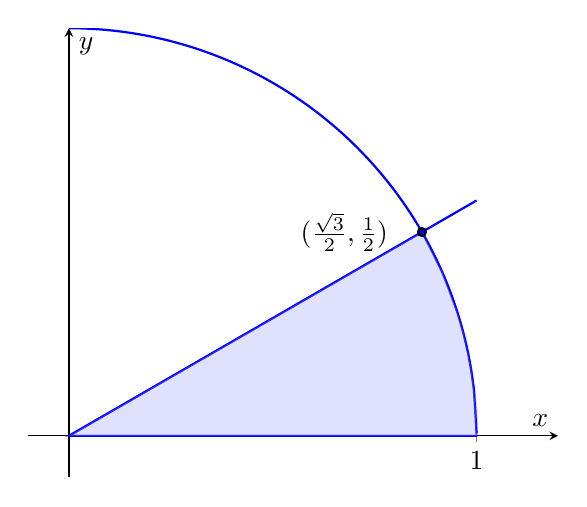
\begin{tikzpicture}
        \begin{axis}[axis lines = center, xtick = {1}, ytick = \empty, 
        ymin = -0.1, ymax = 1, xmin = -0.1, xmax = 1.2, xlabel = $x$, 
        ylabel = $y$, unit vector ratio = 1 1 1]
            \addplot[blue, thick, domain = 0:1, samples = 150]{sqrt(1-x^2)};
            \addplot[blue, thick, domain = 0:1]{x/sqrt(3)};
            \addplot[blue, thick, domain = 0:1]{0};
            \filldraw[blue, thick, fill = blue!30, opacity = 0.4] (0,0) -- 
            (1, 0) -- (0.99875, 0.05) -- (0.99499, 0.1) -- (0.98869, 0.15) -- 
            (0.9798, 0.2) -- (0.96825, 0.25) -- (0.95394, 0.3) -- 
            (0.91652, 0.4) -- (0.866, 0.5) -- cycle;
            \draw[black, thick, fill = blue] (0.866, 0.5) circle (0.05cm) node[
            black, left, xshift = -0.3cm] {$(\frac{\sqrt{3}}{2}, \frac{1}{2})$};
        \end{axis}
    \end{tikzpicture}

    We see that the region defined in polar coordinates is $\textit{D} = \{(r, 
    \theta)\text{ }|\text{ }0 \leq r \leq 1,\text{ }0 \leq \theta \leq \pi/6\}$
    . And therefore:
    $$\int_0^{1/2} \int_{\sqrt{3}y}^{\sqrt{1 - y^2}} xy^2\,dx\,dy = \int_0^{
    \pi/6} \int_0^1 r \left( r \cos{\theta} \right) \left(r \sin{\theta} 
    \right)^2\,dr\,d\theta$$
    $$= \int_0^{\pi/6} \left[ \cos{\theta} \sin^2{\theta} \right]\,d\theta 
    \cdot \int_0^1 r^4 \,dr$$
    $$= \left( \frac{1}{3}\sin^3{\theta}|_{\theta = 0}^{\theta = \pi/6} \right) 
    \cdot \left( \frac{1}{5} r^5 |_{r = 0}^{r = 1}\right)$$
    $$= \frac{1}{15} \cdot \left( \frac{1}{2} \right)^3 = \frac{1}{120}$$

    \item Visualizing the region:
    
    \begin{tikzpicture}
        \begin{axis}[axis lines = center, xtick = {1, 2}, ytick = {1}, 
        xmin = -0.2, xmax = 2.2, ymin = -0.2, ymax = 1.2, unit vector ratio = 
        1 1 1, xlabel = $x$, ylabel = $y$]
            \addplot[name path = A, blue, thick, domain = 0:2, samples = 150]{
            sqrt(2*x - x^2)};
            \addplot[name path = B, blue, thick, domain = 0:2]{0};
            \addplot[blue, fill = blue!30, opacity = 0.4] fill between [
            of = A and B];
        \end{axis}
    \end{tikzpicture}

    We see that the region is the top half of a circle of radius 1 centered at 
    (1, 0). In polar coordinates, this region is $\textit{D} = \{(r, \theta)
    \text{ }|\text{ }0 \leq r \leq 2\cos{\theta}, 0 \leq \theta \leq \pi/2\}$. 
    And therefore:
    $$\int_0^2 \int_0^{\sqrt{2x - x^2}} \sqrt{x^2 + y^2}\,dy\,dx = \int_0^{\pi/
    2} \int_0^{2\cos{\theta}} r \sqrt{r^2}\,dr\,d\theta$$
    $$= \int_0^{\pi/2} \int_{0}^{2\cos{\theta}} r^2\,dr\,d\theta = \int_0^{\pi/
    2} \frac{1}{3} \left[ r^3 \right]_{r = 0}^{r = 2\cos{\theta}}\,d\theta$$
    $$= \frac{8}{3} \int_0^{\pi/2} \cos^3{\theta}\,d\theta = \frac{8}{3} \int_
    0^{\pi/2} \cos{\theta} \left(1 - \sin^2{\theta} \right)\,d\theta$$
    $$= \frac{8}{3} \left[ \int_0^{\pi/2} \cos{\theta}\,d\theta - \int_0^{\pi/2
    } \cos{\theta}\sin^2{\theta}\,d\theta \right]$$
    $$= \frac{8}{3} \left[ \left(\sin{\theta} \right)_{\theta = 0}^{\theta = 
    \pi/2} - \left( \frac{1}{3} \sin^3{\theta} \right)_{\theta = 0}^{\theta = 
    \pi/2} \right]$$
    $$= \frac{8}{3} \left[ \left(1 - 0 \right) - \frac{1}{3} \left( 1^3 - 0^3 
    \right) \right] = \frac{8}{3} \cdot \frac{2}{3} = \frac{16}{9}$$
\end{enumerate}
\end{Answer}

\begin{Exercise}[title={Using Polar Coordinates in Multiple Integration}, 
label=polarmulti]

Find the volume of the solid that lies under the surface $z = 4 - x^2 - y^2$ 
and above the $xy$-plane.
\vspace{50mm}
\end{Exercise}
\begin{Answer}[ref=polarmulti]

We are finding the volume of the solid that lies under the surface $z = 4 - 
x^2 - y^2$ and above the $xy$-plane.

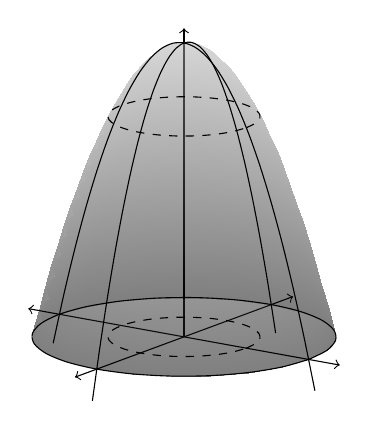
\begin{tikzpicture}
  \begin{axis}[
    view={35}{15},
    unit vector ratio=1 1 1,
    ticks = none,
    axis lines=middle,
    ymin=-2.5,
    ymax=2.5,
    xmax=2.5,
    xmin=-2.5,
    zmin=0,
    zmax=4.2,
    x axis line style=<->,
    y axis line style=<->,
    z axis line style=->,
    clip=false
  ]
    \addplot3[surf,shader=interp,domain=0:360,y domain=0:2, opacity=0.5,
    colormap={blackwhite}{color=(black) color=(black!30)}] ({y*cos(x)},
    {y*sin(x)},{4-y^2});
    \addplot3[samples y=0,domain=0:360,smooth]({2*cos(x)},  {2*sin(x)},0);
    \addplot3[samples y=0,domain=0:360,smooth,dashed]({cos(x)},  {sin(x)},0);
    \addplot3[samples y=0,domain=0:360,smooth,dashed]({cos(x)},  {sin(x)},3);
    \addplot3[samples y=0,domain=-2.1:2.1,smooth](0,  {x},{4 - x^2});
    \addplot3[samples y=0,domain=-2.1:2.1,smooth]({x},0, {4 - x^2});
  \end{axis}
\end{tikzpicture}

We can use polar coordinates to simplify the double integral. In polar 
coordinates, $x = r\cos(\theta)$ and $y = r\sin(\theta)$, so $x^2 + y^2 = r^2$.
The volume under the surface and above the $xy$-plane is given by

\begin{equation}
V = \int \int (4 - r^2) r \, dr \, d\theta,
\end{equation}

where $r$ ranges from 0 to 2 (since $4 - r^2 \geq 0$ if $0 \leq r \leq 2$) and 
$\theta$ ranges from 0 to $2\pi$.

Hence,

\begin{align*}
V & = \int_{0}^{2\pi} \int_{0}^{2} (4r - r^3) \, dr \, d\theta \\
& = \int_{0}^{2\pi} \left[ 2r^2 - \frac{1}{4}r^4 \right]_{0}^{2} \, d\theta \\
& = \int_{0}^{2\pi} (8 - 4) \, d\theta \\
& = \int_{0}^{2\pi} 4 \, d\theta \\
& = \left[ 4\theta \right]_{0}^{2\pi} \\
& = 8\pi.
\end{align*}

So, the volume of the solid is $8\pi$ cubic units.

\end{Answer}

\begin{Exercise}[title = {The volume of a pool}, label = polarmulti2]
A circular swimming pool has a 40-ft diameter. The depth of the pool is 
constant along the north-south axis and increases from 3 feet at the west end 
to 10 feet at the east end. What is the total volume of water in the pool? 
\vspace{50mm}
\end{Exercise}

\begin{Answer}[ref = polarmulti2]
Let's describe the footprint of the pool as a 20-foot radius circle centered 
at the origin (that is, a region \textit{D}$ = \{(r, \theta)\text{ }|\text{ }0 
\leq r \leq 20,\text{ }0 \leq \theta \leq 2\pi\}$). Further, let's take 
north-south as parallel to the y-axis and east-west as parallel to the x-axis. 
So, the depth of water is then given by $z = f(x, y) = \frac{7}{40}x + \frac{
13}{2}$ over the footprint of the pool. The total volume of water is given 
by:
$$\int_0^{2\pi} \int_0^{20} r \left( \frac{7}{40}r\cos{\theta} + \frac{13}{2} 
\right)\,dr\,d\theta$$
$$= \int_0^{2\pi} \int_0^{20} \left[ \frac{7}{40}r^2\cos{\theta} + \frac{13}{2}
r \right] \,dr\,d\theta$$
$$= \int_0^{2\pi} \left[ \frac{7\cos{\theta}}{40}\int_0^{20} r^2\,dr + \frac{13
}{2} \int_0^{20} r\,dr \right]\,d\theta$$
$$= \int_0^{2\pi} \left[ \frac{7\cos{\theta}}{40} \left( \frac{1}{3}r^3 \right)
_{r = 0}^{r = 20} + \frac{13}{2} \left( \frac{1}{2}r^2 \right)_{r = 0}^{r = 20}
\right]\,d\theta$$
$$= \int_0^{2\pi} \left[ \frac{1400}{3}\cos{\theta} + 1300 \right]\,d\theta = 
\left[ \frac{1400}{3}\sin{\theta} + 1300\theta \right]_{\theta = 0}^{\theta = 
2\pi}$$
$$= 2600\pi \text{ cubic feet}$$    
\end{Answer}
